\chapter{Odkrivanje skupin}

Odkrivanje skupin, ali razvrščanje podatkov v skupine, je ena od
osnovnih tehnik podatkovne analitike. Na podlagi podatkov o
uporabnikih marketinški oddelek lahko zanima segmentacija uporabnikov,
oziroma kateri so njihovi tipični uporabniki in koliko takih skupin
sploh imajo. Poznavanje skupin in njihovih lastnosti lahko privede do
izdelave boljših ciljnih akcij. Na področju medicine nas lahko
zanimajo tipične skupine bolnikov, da bi lahko njim prilagodili in
izboljšali bolnišnični sistem. Raziskovalce vesolja lahko zanima,
kakšne skupine galaksij (poleg teh, ki so jih že odkrili) poznamo in
predvsem, kakšne so njihove karakteristike. V množici dokumentov nas
mnogokrat lahko razveseli, če lahko z algoritmi odkrijemo skupine med
seboj podobnih enot in uporabnikom na ta način olajšamo brskanje po
gradivu. Fotografu lahko pomagamo, če mu s pomočjo računalnika
uredimo slikovno gradivo, ki ga je v zadnjem desetletju nakopičil na
zunanjem disku. Iz podatkov o odnosih šolskimi otroci šolske sociologe
mnogokrat zanima oblikovanje skupin, pa tudi odkrivanje osamelcev, ki
jim je potrebno pomagati pri socializaciji. Različnih uporab tehnik
odkrivanja skupin je mnogo in vsekakor preveč, da bi jih tu vse
našteli, zato raje pričnemo s primerom.

\section{Primer podatkov}

V razredu 8.A je šestnajst učencev, ki jih je šolski sistem ravno
izmučil z republiškim eksternim preverjanjem znanja. Uspeh, ki so ga
dosegli, je podan v tabeli~\ref{t-eksterci}. Številke so percentili;
Branka je na primer bila dobra pri angleščini, kjer je bila boljša od
95 odstotkov vseh učencev, ki so pisali test. Ni pa ji ravno šla
fizika, kjer je bilo slabših od nje le 11 odstotkov.

\begin{table}[htbp]
\caption{Rezultati zunanjega preverjanja za 16 učencev razreda 8.A. Rezultati
  posameznih predmetov so podani v percentilih z ozirom na republiške
  rezultate.}
\label{t-eksterci}
\begin{center}
\begin{tabular}{lrrrrrrrrr}
\toprule
ime & slo & ang & zgo & geo & mat & bio & fiz & kem & tel \\
\midrule
Albert & 22 & 81 & 32 & 39 & 21 & 37 & 46 & 36 & 99 \\
Branka & 91 & 95 & 65 & 96 & 89 & 39 & 11 & 22 & 29 \\
Cene & 51 & 89 & 21 & 39 & 100 & 59 & 100 & 89 & 27 \\
Dea & 9 & 80 & 18 & 34 & 61 & 100 & 90 & 92 & 8 \\
Edo & 93 & 99 & 39 & 100 & 12 & 47 & 17 & 12 & 63 \\
Franci & 49 & 83 & 17 & 33 & 92 & 30 & 98 & 91 & 73 \\
Helena & 91 & 99 & 97 & 89 & 49 & 96 & 81 & 94 & 69 \\
Ivan & 12 & 69 & 32 & 14 & 34 & 12 & 33 & 48 & 96 \\
Jana & 91 & 80 & 20 & 10 & 82 & 93 & 87 & 91 & 22 \\
Leon & 39 & 100 & 19 & 29 & 99 & 31 & 77 & 79 & 23 \\
Metka & 20 & 91 & 10 & 15 & 71 & 99 & 78 & 93 & 12 \\
Nika & 90 & 60 & 45 & 34 & 45 & 20 & 15 & 5 & 100 \\
Polona & 100 & 98 & 97 & 89 & 32 & 72 & 22 & 13 & 37 \\
Rajko & 14 & 4 & 15 & 27 & 61 & 42 & 51 & 52 & 39 \\
Stane & 9 & 22 & 8 & 7 & 100 & 11 & 92 & 96 & 29 \\
Zala & 85 & 90 & 100 & 99 & 45 & 38 & 92 & 67 & 21 \\
\bottomrule
\end{tabular}
\end{center}
\end{table}

Zanima nas, ali so v razredu kakšne značilne skupine učencev in če so,
kakšne so njihove karakteristike oziroma kako se razlikujejo med
sabo. Zanima nas tudi, kateri učenci so si med sabo podobni. Spoznanja
na tem področju bodo šoli pomagala pri oblikovanju skupin, kjer bi na
primer skupini, ki je dobra v naravoslovnih predmetih slaba pa pri
slovenščini posebej poiskali kakšno zanimivo knjigo za domače branje,
te, ki pa jim gre družboslovje, navdušili za novinarski krožek.

\section{Nekaj matematičnih oznak}

Učencem iz tabele~\ref{t-eksterci} bomo rekli učni primeri in jih bomo
označili z $x^{(i)}$, kjer je $i$ indeks primera. Ker se bomo na teh
primerih skušali naučiti, kakšne skupine poznamo v razredu 8.A, bomo
tem primerom rekli učni primeri. Množico učnih primerov označimo z
$\mathcal{U}$, njeno moč oziroma število primerov pa označimo z $m$,
torej $m=|\mathcal{U}|$. Naj bo $C\subset \mathcal{U}$ skupina
primerov, $\mathcal{C}=\{C_j\}$ pa razvrstitev, to je množica skupin,
ki smo jo odkrili v podatkih. Tu se bomo ukvarjali samo s postopki, ki
odkrivajo neprazne skupine, $|C_i|>0$. Zanimali nas bodo različni tipi
razvrstitev. Možna razvrstitev je lahko takšna, kjer si skupine med
seboj ne delijo nobenega primera,
%
$$C_i\cap C_j=\emptyset;\ C_i,C_j\in\mathcal{C}$$
%
in kjer je unija vseh skupin enaka učni množici,
%
$$ \displaystyle\bigcup_{C_i\in\mathcal{C}}C_i=\mathcal{U} $$ 
%
Pri taki razvrstitvi torej vsak primer pripada natanko eni
skupini. Tako razvrstitev imenujemo razbitje.

Zanimale nas bodo tudi hierarhije skupin, kjer velja $C_i\cap
C_j\in\{C_i,C_j,\emptyset\}$.  Presek dveh skupin je lahko samo prazna
množica, ali pa v celoti ena od skupin. Pri nepraznem preseku to
pomeni, da je ena od skupin v celoti vsebovana v drugi. Tako lastnost
bodo imele skupine v pri hierarhičnem razvrščanju.

Vsak primer tabeli~\ref{t-eksterci} je opisan z $n$ atributi
(številskimi spremenljivkami). Primer $x$ zapišemo kot:
%
$$ x=(x_1,x_2, \ldots, x_n)^T $$ 
%
Tu smo zaradi poenostavitve namenoma izpustili indeks primera. Primer
$x^{(i)}$ smo tako označili s simbolom $x$. Ker je vsak primer vektor,
bi temo primerno morali izpisati tudi oznako, torej kot $\bf x$, a
bomo tudi poenostavili in primer označili kar z $x$.

Primer smo zapisali kot stolpični vektor, v tabeli s primeri pa je
zapisan kot vrstični vektor, ki ga zato, da dobimo stolpec,
transponiramo. Pravzaprav je to, ali je primer zapisan kot stolpec ali
vrstica, za sedaj precej nepomembno, bo pa notacija pomembna takrat,
kadar bomo o naboru primerov razmišljali kot o matriki. Primeri v naši
tabeli so poimenovani (imena učencev), atributi pa imajo prav tako
ime. Lahko bi sicer za naš primer Albert pisali
$x^{(Albert)}_{slo}=22$, a bomo v nadaljevanju zaradi splošnosti raje
uporabljali numerične indekse.

\section{Mere različnosti}

V postopku odkrivanja skupin primerov bi želeli poiskati množice
primerov, kjer so si ti med seboj čim bolj podobni. Oziroma
enakovredno, vsebujejo primere, kjer so si ti med sabo čimmanj
različni. Tu nam bo torej prav prišla mera različnosti. Najbolj
enostavno je pričeti s parom primerov in za ta zapisati enačbo, s
katero ocenimo, kako različna sta. Vzemimo primera $a$ in $b$ in
predpostavimo, da sta ta opisana z atributi, ki lahko zavzamejo zvezne
vrednosti:
%
$$ a = (a_1,a_2, \ldots, a_n) $$
$$ b = (b_1,b_2, \ldots, b_n) $$
%
Tu bi lahko primera označil z $x^{(a)}$ in $x^{(b)}$, a bi potem
enačbe, ki sledijo, dobile nepotrebno prtljago.

Če si predstavljamo, da je domenski atributni prostor Evklidski, potem
je primerna razdalja oziroma mera različnosti med primeri kar
evklidska razdalja:
$$ d(a,b)=\sqrt{\sum_{i=1}^n(a_i-b_i)^2} $$ 
%
Kako bi najbolj enostavno izmerili razdalje med primeri za $n=2$ in za
primere, ki jih v ta namen izrišemo na milimetrski papir? Z drugimi
besedami, kako bi izmerili razdalje med primeri v razsevnem diagramu?
Z ravnilom. Zato razdalji, ki je opisana z zgornjo enačbo, rečemo
Evklidska.

Še enostavnejša je Manhattanska razdalja (od kod in zakaj to ime?):
$$ d(a,b)={\sum_{i=1}^n|\ a_i-b_i\ |} $$
Obe, Manhattanska in Evklidska razdalja pa sta posebni primer razdalje
Minkowskega:
$$ d(a,b)=({\sum_{i=1}^n|a_i-b_i|^r})^{\frac{1}{r}} $$

O merah različnosti bomo še govorili. Premisliti bo na primer še
potrebno, kako merimo razdalje pri različnih tipih atributov. Na
primer, če ti zavzemajo diskretne vrednosti. Ali pa kako merimo
razdalje med besedili in nizi znakov, med dokumenti, med stvarmi v
priporočilnih sistemih, med slikami, med glasbenimi posnetki in
podobno. A za naš primer so zgornje definicije dovolj.

Z izbrano mero različnosti lahko izmerimo razdalje med vsemi
pari primerov. Te potem lahko vizualiziramo s toplotno karto
(\angl{heatmap}), kot to prikazuje slika~\ref{f-toplotna-karta}. Če
``močne'' skupine obstajajo, in če smo primere na toplotni karti
pravilno uredili (kako?), bi se na karti morali prikazati vzorci, ki
nakazujejo skupine (kakšni?).

\begin{figure}[htbp]
\begin{center}
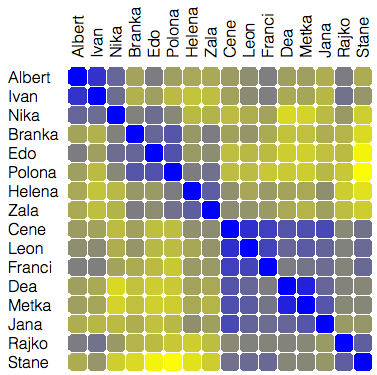
\includegraphics[width=7cm]{slike/toplotna-karta.png}
\caption{Vizualizacija podobnosti oziroma različnosti med primeri s
  tabele~\ref{t-eksterci}.}
\label{f-toplotna-karta}
\end{center}
\end{figure}

\section{Ocenjevanje razdalj med skupinami}

Tudi med skupinami primerov lahko merimo razdaljo. A tu naletimo na
problem, saj so sedaj skupine podane z množico primerov. Med primeri
znamo meriti razdalje, med skupinami pa (še) ne. Razdaljo bomo merili
med dvemi skupinami primerov, $C_u$ in $C_v$. Predpostavimo najprej,
da si skupine ne delijo primerov, torej $C_u\cap
C_v=\emptyset$. Uvedimo nekaj možnih razdalj:
\begin{itemize}
\item Razdalja med skupinama $C_u$ in $C_v$ je razdalja med njunima
  najbližjima primeroma $a\in C_u$ in $b\in C_v$ \angl{single
    linkage}:
$$d_{\rm min}(C_u, C_v)=\min_{a,b}\{d(a,b)\ |\ a\in C_i, y\in C_j\}$$
\item Razdalja med skupinama $C_u$ in $C_v$ je razdalja med njunima
  najbolj oddaljenima primeroma $a\in C_u$ in $b\in C_v$
  \angl{complete linkage}:
$$d(C_{\rm max}, C_v)=\max_{a,b}\{d(a,b)\ |\ a\in C_i, b\in C_j\}$$
\item Razdalja med skupinama $C_u$ in $C_v$ je povprečna razdalja med
  vsemi pari primerov iz teh dveh skupin \angl{average linkage}, torej:
$$d(C_u, C_v)={\sum_{a\in C_u}\sum_{b\in C_v}  \frac{d(a,b)}{|C_a||C_b|}} $$
\item Wardova razdalja, ki privzame, da je za vsako skupino $C$ znan
  njen centroid $R$ oziroma točka v središču skupine. Naj bo $R_u$
  centroid skupine $C_u$, $R_v$
  centroid skupine $C_v$, $R_{uv}$ pa centroid združene skupine
  $C_{uv}=C_u\cup C_v$. Potem je Wardova razdalja določena kot:
$$d_w(C_u, C_v)=\sum_{x\in C_{uv}}d(x, R_{uv})^2 - (\sum_{x\in
    C_u}d(x, R_u)^2 + \sum_{x\in C_v}d(a, R_v)^2)$$
\end{itemize}

\section{Hierarhično razvrščanje v skupine}

Postopek, ki iz podatkov razvije hierarhijo skupin, kjer je najnižje v
hierarhiji vsak primer predstavljen s svojo skupino, najvišje v
hierarhiji pa tvori skupino kar celotna množica učnih primerov, se
imenuje hierarhično razvrščanje v skupine.

\subsection{Algoritem}

Hierarhično razvrščanje v skupinenajlažje opišemo kar s psevdokodo:
\begin{itemize}
\item vsak primer naj tvori svojo skupino, $C_i=\{x^{(i)}\}$,
  $x^{(i)}\in\mathcal{U}$
\item ponavljaj, dokler ne ostane ena sama skupina
\begin{itemize}
\item poišči najbližji si skupini $C_a$ in $C_b$,
  $d(C_a,C_b)=\min_{u,v}d(C_u,C_v)$
\item združi skupini $C_a$ in $C_b$ v skupino $C_{ab}=C_a\cup
  C_b$
\item nadomesti skupini $C_a$ in $C_b$ s skupino $C_{ab}$
\item izmeri razdaljo med novo skupino $C_{ab}$ in ostalimi skupinami
\end{itemize}
\end{itemize}

Prostorska kompleksnost tega algoritma je $O(m^2)$, kjer je $m$
število primerov oziroma velikost učne množice. Časovna kompleksnost
pa je $O(m^3)$ saj se algoritem izvede v $m$ korakih, v katerih mora
osvežiti in uporabiti matriko razdalj velikosti $m^2$. Z malo truda se
da postopek izračunavanja novih razdalj spisati tako, da ima manjšo
zahtevnost in je potem zahtevnost celotnega algoritma
$O(m^2\log(m))$. Tudi to ni malo. Predstavljajte si, da morate
algoritem pognati na vseh uporabnikih nekega večjega mobilnega
operaterja. Ali pa na vseh uporabnikih družabnega omrežja. Kam
shranite matriko razdalj med pari primerov? Je opisani postopek tudi
časovno zahteven?

\subsection{Dendrogram}

Postopek združevanja v skupine in rezultat tega postopka ---
hierarhijo skupin, lahko ponazorimo v drevesnem izrisu ali dendrogramu
(gr. {\em dendron} pomeni drevo, {\em gramma} pa risba). Dendrogram
hierarhičnega razvrščanja v skupine podatkov s tabele~\ref{t-eksterci}
prikazuje slika~\ref{f-dendrogram}. Dendrogram je izrisan od leve
proti desni. Stičišča skupin so od desnega roba odmaknjena skladno z
razdaljo med skupinami. Pred izvedbo postopka razvrščanja v skupine
orodja podatke tipično normalizirajo, tako da so po normalizaciji
povprečne vrednosti atributov enake nič in njihove standardne
deviacije enake 1.

\begin{figure}[htbp]
\begin{center}
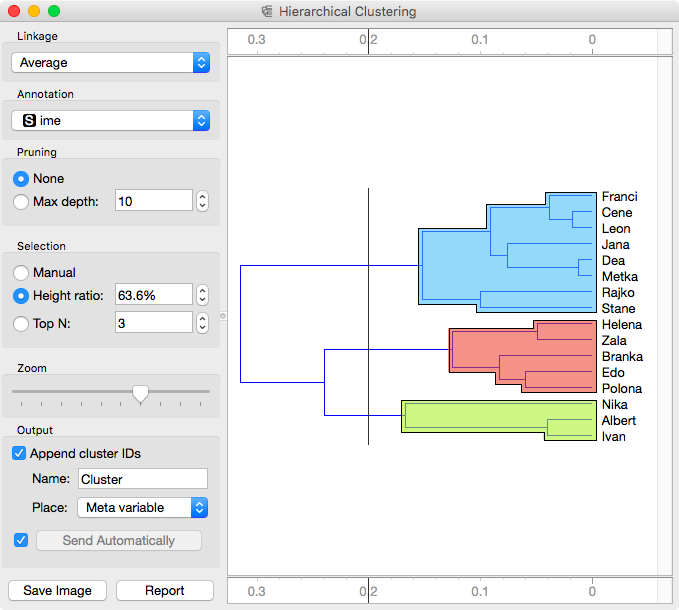
\includegraphics[width=10cm]{slike/dendrogram.png}
\caption{Primer dendrograma, kot ga izriše ustrezna komponenta v
  programu Orange. Uporabnik se je tu odločil, da dendrogram odreže v
  točki, ki primere razdeli v tri skupine. Primerna razdelitev v
  tem primeru bi lahko bila ta, ki uporabi dve skupine. Zakaj?}
\label{f-dendrogram}
\end{center}
\end{figure}

\subsection{Razlaga skupin}

Dendrogram s slike~\ref{f-dendrogram} nakazuje na tri skupine, ki smo
jih v odkrili v podatkih. Zanima nas, kaj je značilnega za posamezne
skupine. Preprosta tehnika, ki jo lahko uporabimo je, da za vsak
skupino primerjamo povprečno
vrednost posameznega atributa s povprečno vrednostjo tega atributa v
celotni učni množici. Naj bo Albert v skupini, ki jo označimo z
vrstnim številom 1, Branka v skupini 2, Cene pa v skupini 3. Povprečne
vrednosti učne množice prikazuje tabela~\ref{f-povp-skupin}.

\begin{table}[htbp]
\caption{Povprečne vrednosti percentilov pri posameznih predmetih v
  učni množici in odkritih skupinah.}
\label{f-povp-skupin}
\begin{center}
\begin{tabular}{lrrrrrrrrr}
\toprule
 & slo & ang & zgo & geo & mat & bio & fiz & kem & tel \\
\midrule
$\mathcal{U}$ & 54 & 78 & 40 & 47 & 62 & 52 & 62 & 61 & 47 \\
skupina 1 & 41 & 70 & 36 & 29 & 33 & 23 & 31 & 30 & 98 \\
skupina 2 & 92 & 96 & 80 & 95 & 45 & 58 & 45 & 42 & 44 \\
skupina 3 & 35 & 69 & 16 & 24 & 83 & 58 & 84 & 85 & 29 \\
\bottomrule
\end{tabular}
\end{center}
\end{table}

Zanima nas pravzaprav odstopanje od povprečnih vrednosti atributov
učne množice. Tu bi se sicer morali poigrati s statistiko, in
ugotoviti, katera odstopanja so značilna in kako daleč so od takih, ki
bi jih dobili iz naključne razvrstitve. Zaradi enostavnosti, ki pa bo
prav tako čisto primerna za naš primer, se tu raje zatečemo
k veliko preprostejši rešitvi. Za vsako skupino označimo odstopanja
navzdol za več kot 10 odstotnih točk z ``$-$'', in podobna odstopanja
navzgor s ``+''. 

\begin{table}[htbp]
\caption{Odstopanja ($\pm 10$ točk) od povprečnih vrednosti v učni množici.}
\label{f-odstopanja-skupin}
\begin{center}
\begin{tabular}{lcccccccccc}
\toprule
 & slo & ang & zgo & geo & mat & bio & fiz & kem & tel \\
\midrule
skupina 1 & $-$ &  &  & $-$ & $-$ & $-$ & $-$ & $-$ & + \\
skupina 2 & + & + & + & + & $-$ &  & $-$ & $-$ &  \\
skupina 3 & $-$ &  & $-$ & $-$ & + &  & + & + & $-$ \\
\bottomrule
\end{tabular}
\end{center}
\end{table}

Rezultat prikazuje tabela~\ref{f-odstopanja-skupin}. Albert, Ivan in
Nika so kot kaže športniki. Njihovo udejstvovanje s športom jim vzame
veliko časa, morda bi jim bilo potrebno pomagati pri naravoslovnih
predmetih, kjer jim malce škripa. Branka, Edo in ostali iz skupine 2
imajo rajši družboslovne predmete. Skupina s Cenetom, Deo in Metko pa
zanima naravoslovje. Ne bi bilo narobe, če bi se ti vpisali v kakšen
športni krožek.

\subsection{Stvari pa lahko tudi obrnemo}

Namesto skupin učencev nas bi lahko zanimale tudi skupine
predmetov. Kako? Tabelo podatkov enostavno zasukamo oziroma
transponiramo. Vse ostalo ostane isto. Rezultat je podan na
sliki~\ref{f-dendrogram-predmeti}.

\begin{figure}[htbp]
\begin{center}
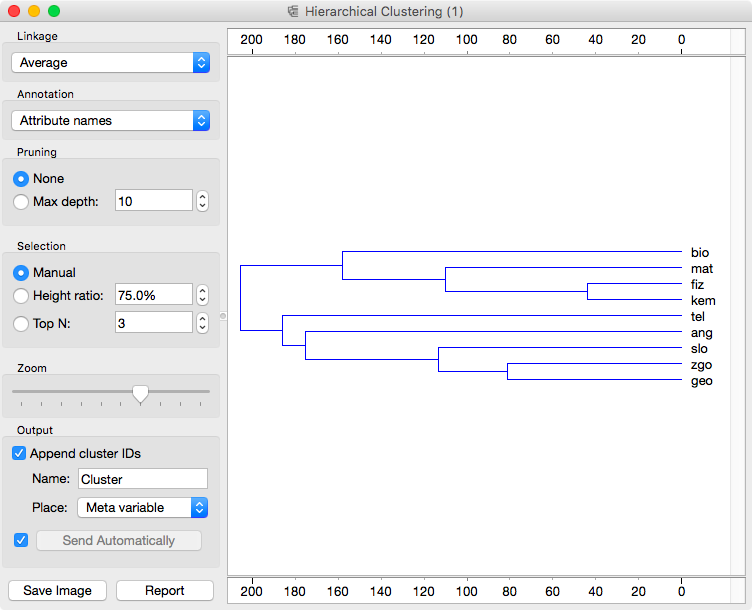
\includegraphics[width=10cm]{slike/dendrogram-predmeti.png}
\caption{Dendrogram skupin predmetov. Telovadba je nekakšen osamelec,
  samosvoj predmet precej različen od ostalih. Kako je to vidno iz
  dendrograma?}
\label{f-dendrogram-predmeti}
\end{center}
\end{figure}

\subsection{Kaj pa, ko ni skupin?}

Hierarhično razvrščanje v skupine bo vedno našlo skupine. Postopek bo
vedno razvil dendrogram, ne glede na to, ali skupine dejansko
obstajajo v podatkih ali ne. Pravzaprav, kaj pa so sploh skupine? Kako
lahko sploh ocenimo, ali te dejansko obstajajo? Tole se v tem trenutku
precej težka vprašanja in se bomo z njimi še ukvarjali. A vseeno, za
okus, naredimo naslednji poskus. Naše podatke o ocenah učencev 8.A
razreda uničimo tako, da naključno premešamo števila v vsaki od kolon,
za vsako kolono posebej. Dendrogram na takih podatkih kaže
slika~\ref{f-dendrogram-premesano}. Razdalje med posameznimi skupinami
so tu večje, stičišča povezav v dendrogramu so se premaknila proti
levi strani. Stukture, iz katere bi bile jasno razvidne skupine, ki bi
se potem združevale pri opazno večjih razdaljah kot se združujejo
primeri znotraj posameznih skupin, ni več.

\begin{figure}[htbp]
\begin{center}
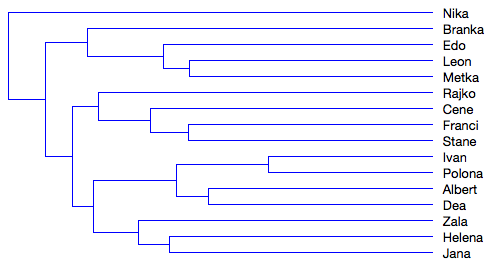
\includegraphics[width=10cm]{slike/dendrogram-premesano.png}
\caption{Dendrogram na ``ponaključenih'' podatkih. Struktura, ki bi
  nakazovala jasne skupine v podatkih, je izginila.}
\label{f-dendrogram-premesano}
\end{center}
\end{figure}

Če imamo prave podatke, te seveda ne premešamo in potem izrisujemo
``pokvarjene'' dendrograme (ali pač? a o pomenu postopkov, ki
temeljijo na ponaključenih podatkih, kdaj drugič). A je vseeno dobro
vedeti, kakšni dendrogrami so taki, kjer skupin pač ni. Torej, če
dobimo kaj podobnega, kot je dendrogram na
sliki~\ref{f-dendrogram-premesano}, je zaključek tak, da iz danih
podatkov pri dani meri razdalje in pri dani metodi za ocenjevanje
razdalj med skupinami postopek hierarhičnega razvrščanja v skupine ni
našel značilnih skupin. Prejšnji stavek je precej dolg. Krajši bi
recimo lahko samo povedal, da v podatkih ni skupin. A taka ugotovitev
ne bi bila nujno resnična. Iz naših poskusov lahko samo ugotovimo, da
če morda skupino so, jih mi pač nismo uspeli najti. Lahko pa, seveda,
da jih sploh ni.

\section{O izboru mer razdalje}

Metoda hierarhičnega gručenja ima pravzaprav dva parametra: prvi je metoda merjenja razdalj med primeri, drugi pa način določanja razdalj med skupinami. Ko imamo podatke predstavljene atributno, torej v tabeli, kjer je vsak primer predstavljen z vektorjem atributnih vrednosti, je evklidska razdalja čisto primerna mera. Če atributi izvirajo na primer iz tekstovnih podatkov in je teh veliko, se izkaže, da je pomembna ne toliko velikost posameznega vektorja kot njegova smer. Prava razdalja za take podatke je tako imenovana kosinusna razdalja. O uporabi te več v naslednjih poglavjih. Na področju biomedicine, kjer so atributi istega tipa in je bolj kot njihova vrednost pomemben vrstni red (tipa: kateri atribut je zavzel največjo vrednost, drugo največjo, ipd.) je mnogokrat uporabljana razdalja Spearmanova korelacija, ki jo izračunamo na rangi. V tem odstavku nam ni namen formalno uvesti vse te različne mere, ampak samo poudariti, da je izbor mere razdalje med primeri odvisen od problemske domene in jo določimo skladno z vedenjem oziroma intuicijo o tem, kaj res najbolj primerno določa razdaljo med primeri.

Malce drugače je z izborom pristopov merjenja razdalje med skupinami. Kot smo že zapisali, ti pristopi (npr. {\em single linkage}, {\em complete linkage}) agregirajo pare razdalj med primeri v dveh različnih skupinah. V splošnem, če ne poznamo podatkov ali pa njihovih projekcij v nižje dimenzije, bo primerna izbira povprečne razdalje \angl{average linkage}, mnogokrat pa presenetljivo dobro deluje Wardova razdalja. Po drugi strani je pristop z minimalno razdaljo \angl.{single linkage} v splošnem neuporaben, razen za res posebne primere (slika~\ref{f-single-linkage}).

\begin{figure}[htbp]
\begin{center}
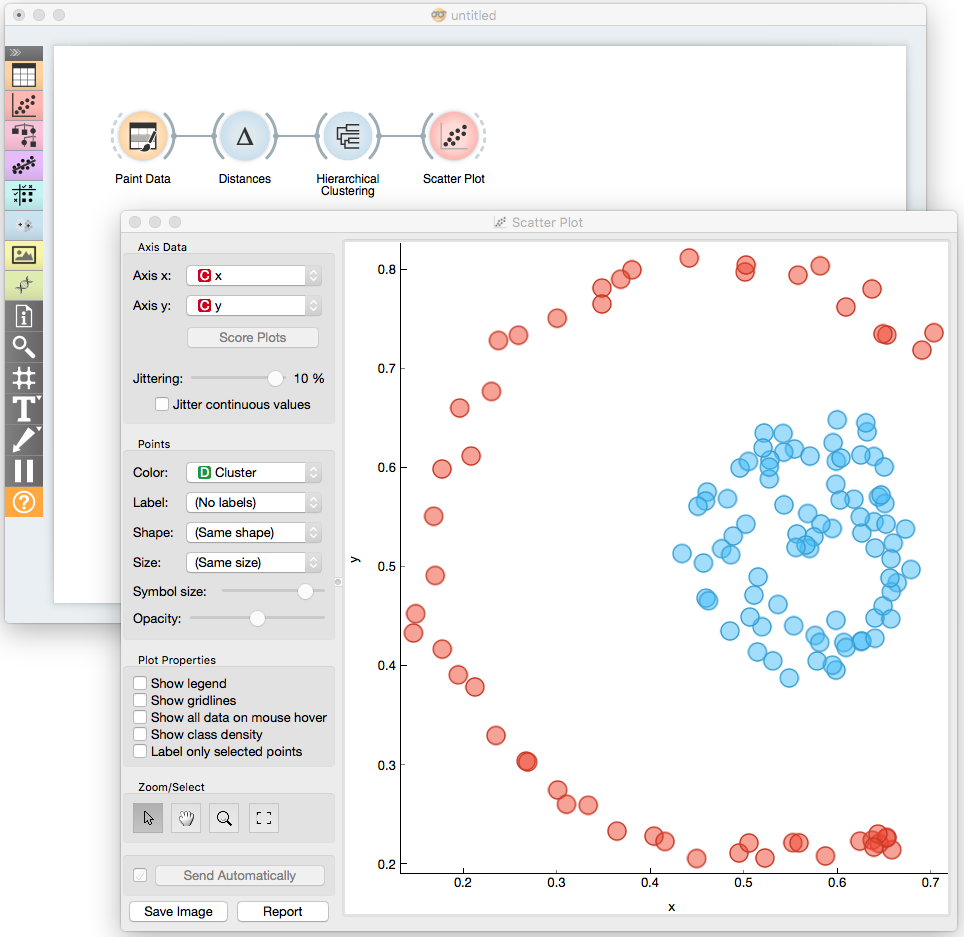
\includegraphics[width=10cm]{slike/single-linkage.png}
\caption{Primer dvodimenzionalnih podatkov in njihove razvrstitve, kjer je ustrezna metoda minimalne razdalje za merjenje podobnosti med skupinami, in kjer ostale metode merjenja razdalj odpovedo (za merjenje razdalj med primeri smo uporabili Evklidsko razdaljo).}
\label{f-single-linkage}
\end{center}
\end{figure}

Recepta, katere mere razdalj uporabiti, v zgodnjih dveh odstavkih nismo zapisali. Ker tega ne znamo. Namreč, vse je odvisno od podatkov. Ker na področju razvrščanja v skupine nimam prav dobrih mer o tem, kako dober je rezultat razvrščanja, se avtomatizacija iskanja najbolj ustreznih parametrov ne obnese najbolje. Z drugimi besedami: v splošnem ne znamo spisati enačbe, s katero bi numerično ocenili kvaliteto nastalih skupin. Ker te enačbe ni, ne moremo strojno primerjati rešitve med sabo. Ostane nam, da se zanesemo na intuicijo in na pregled rešitve s strani domenskega eksperta. Gručenje, ki je uporabniku koristno (za karkoli že), je potem tisto, za katero se na koncu odločimo.
